\section{Background validation}
\label{sec:bkg-val-regns}

\begin{itemize}
	\item Smth about inverting \emph{all} of the cuts?
	\item Since the focus of my thesis was the ggF analysis and , I will share the results from that. Also, since the VBF analysis is so statistically dominated, it was easier to see closure just because the stats were so much lower.
	\item Emphasize how each of these procedures results in retraining all of the NNs for the bootstrap and CR1,2 shape difference
	\item Maybe emphasize how the 3b1f systematic is not included in these studies
\end{itemize}

\begin{figure}[hb]
	\centering
	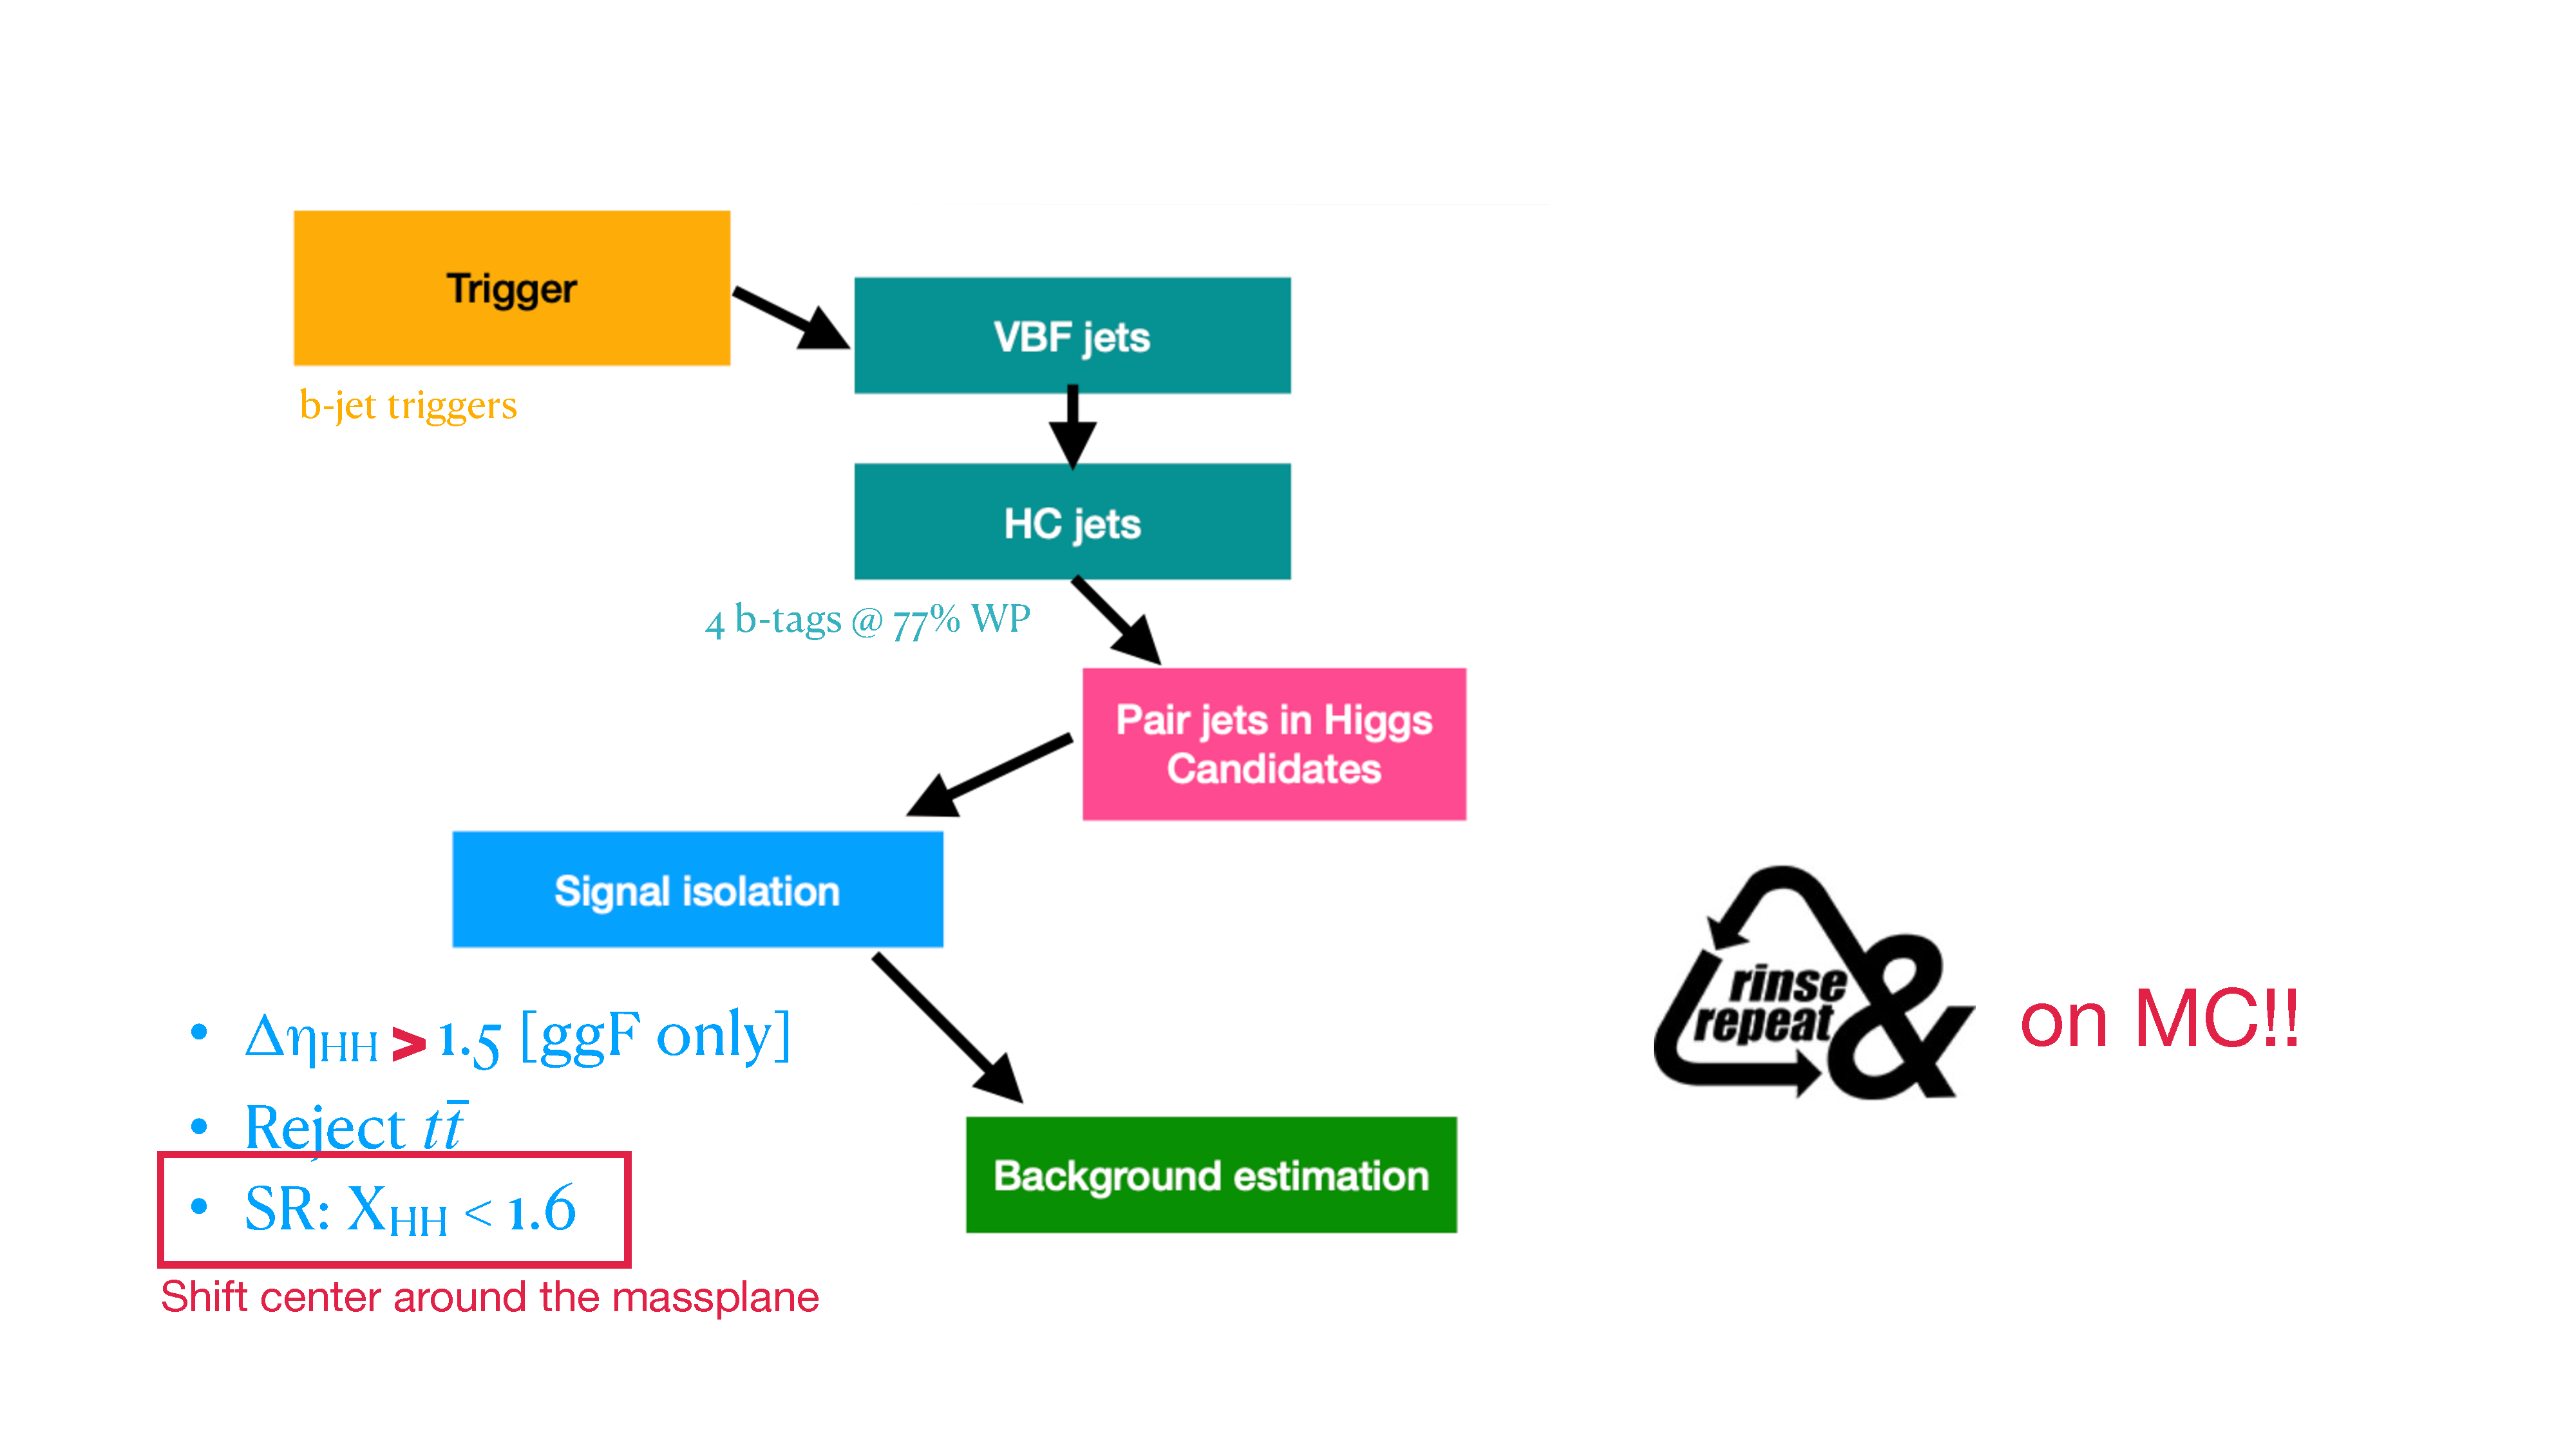
\includegraphics[trim={0 3cm 0 3cm},clip,width=\textwidth]{{figures/my_dihiggs/analysis-validation-graphic.pdf}}
	\caption{Illustration of the modified cuts to test the background estimate strategy.}
	\label{fig:analysis-val}
\end{figure}

\subsection{Reversed  $|\Delta \eta_{HH}|$}


\begin{itemize}
	\setlength\itemsep{0em}
	\item $1.5 < |\Delta \eta_{HH}| < 2.5$
	\item $2.5 <  |\Delta \eta_{HH}| < 3.6$
	\item $|\Delta \eta_{HH}| > 3.6$
\end{itemize}


\def\figpath{figures/nr-int-note/bkgvalidation/V2}

\FloatBarrier
\clearpage
\subsection{Shifted regions}

Another check that we tried was taking the signal region and moving it around the massplane.
Since the equation for the SR defining variable $ \Xhh =  \sqrt{\left(\frac{m_{\PH1} - \SI{124}{\GeV}}{0.1 \ m_{\PH1}}\right)^{2} + \left(\frac{m_{\PH2} - \SI{117}{\GeV}}{0.1 \ m_{\PH2}}\right)^{2}} $  (introduced in \Eq{\ref{eq:xhh}}) has a radius that depends on the $m_{\PH1}$, $m_{\PH2}$, so just changing the center locations had the effect that the SR area got larger as we moved to larger HC masses, as shown in \Fig{\ref{}}. To ameliorate this effect, we modified the HC resolutions in the \Xhh formula so that the SR size would be compatible with the nominal as we moved around the massplane:

\begin{figure}
\centering
\subfloat[Just shift the centers of $X_{hh}$]{
	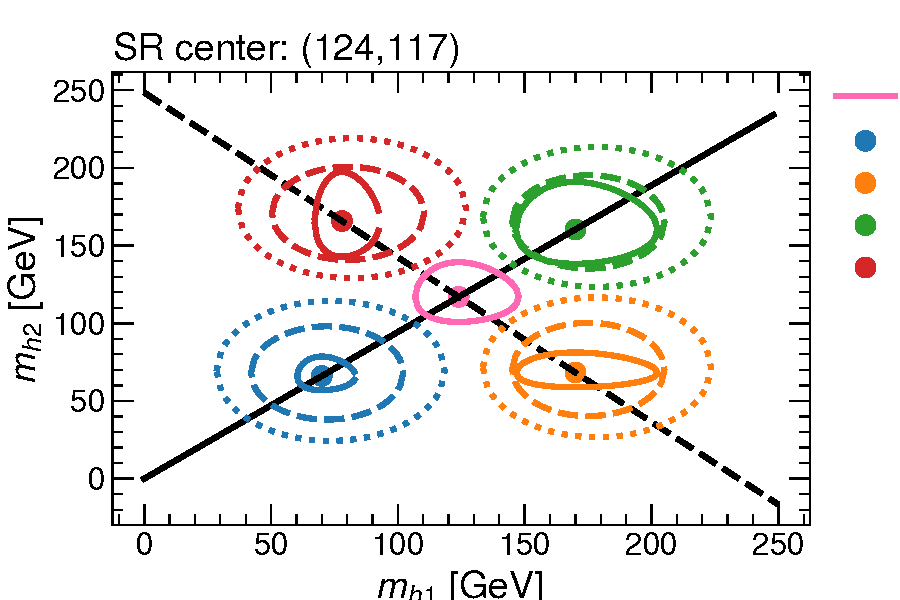
\includegraphics[width=.44\textwidth,trim={0 0 1cm 0},clip]{{figures/my_dihiggs/Xhh_val/onlyShift}}
	\label{fig:Xhh-onlyShift}
	}
\subfloat[$X_{hh}^{shift}$ definition]{
	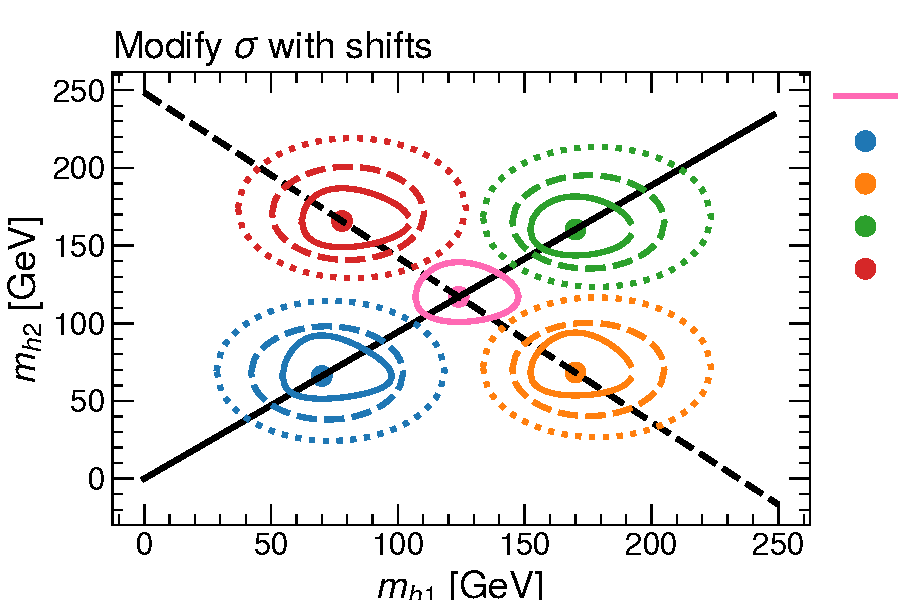
\includegraphics[width=.44\textwidth,trim={0 0 1cm 0},clip]{{figures/my_dihiggs/Xhh_val/newRegions}}
	\label{fig:Xhh-newRegions}
	}
\caption{Motivation for choices of shifted SRs.}
\end{figure}


\begin{equation}
    X_{hh,\mathrm{shift}} = \sqrt{\left(\frac{m_{\PH1} - m_{\PH1,\mathrm{center}}}{\sigma_{m_{\PH1}} \ m_{\PH1}}\right)^{2} + \left(\frac{m_{\PH2} - m_{\PH2,\mathrm{center}}}{\sigma_{m_{\PH2}} \ m_{\PH2}}\right)^{2}}
    \label{eq:shifted-xhh}
\end{equation}

\begin{equation*}
    \text{with} \quad
    \sigma_{m_{\PH1}} = 0.1 \times \frac{124}{m_{\PH1,\mathrm{center}}}, \quad
    \sigma_{m_{\PH2}} = 0.1 \times \frac{117}{m_{\PH2,\mathrm{center}}}.
    \label{eq:shifted-reso-mass}
\end{equation*}

This modification allowed the shifted regions to have approximately equal areas with the standard signal region, as seen in \Fig{\ref{Xhh-newRegions}}.
Although we originally tested SRs that translated both with higher and lower HC masses, we did not have good closure for the reweighting with the ``lower left'' SR. 
We believed understand this because by examining \Fig{\ref{fig:shifted-regions}}, a SR at (70,66)~GeV has CRs that are overlapping the kinematic turn on curve in the massplane. Our intuition tells us that it's harder to form a reliable background estimate if the underlying control region is not smoothly varying into the CR, so we believed that failing to reweight in this region was not a methodological issue, but rather a task that was significantly more difficult than our nominal estimate.
 
The boundary of the CRs just rotates with the center of the SR, and the quadrants are defined in a similar way, as illustrated in \Fig{\ref{Xhh-newRegions}}.
One interesting note is for the lower right SR, the lower quadrant for CR1 has a couple of issues. It (1) intersects with the W-veto from the \Xwt cut and (2) overlaps the kinematic threshold since basically no $m_{\PH 2}$ values below 25~GeV to populate the full lower quadrant.
However, the CR2 (left, right) quadrants did not suffer from these two issues (which made the test more challenging than we believed our actual SR is), so in the following the CR2 derived weights are shown as the nominal set. 
\Tab{\ref{tab:shift-sr-centers}} enumerates of the shifted SR centers and which CR is taken to be the nominal set. 

\begin{figure}[ht]
  \centering
  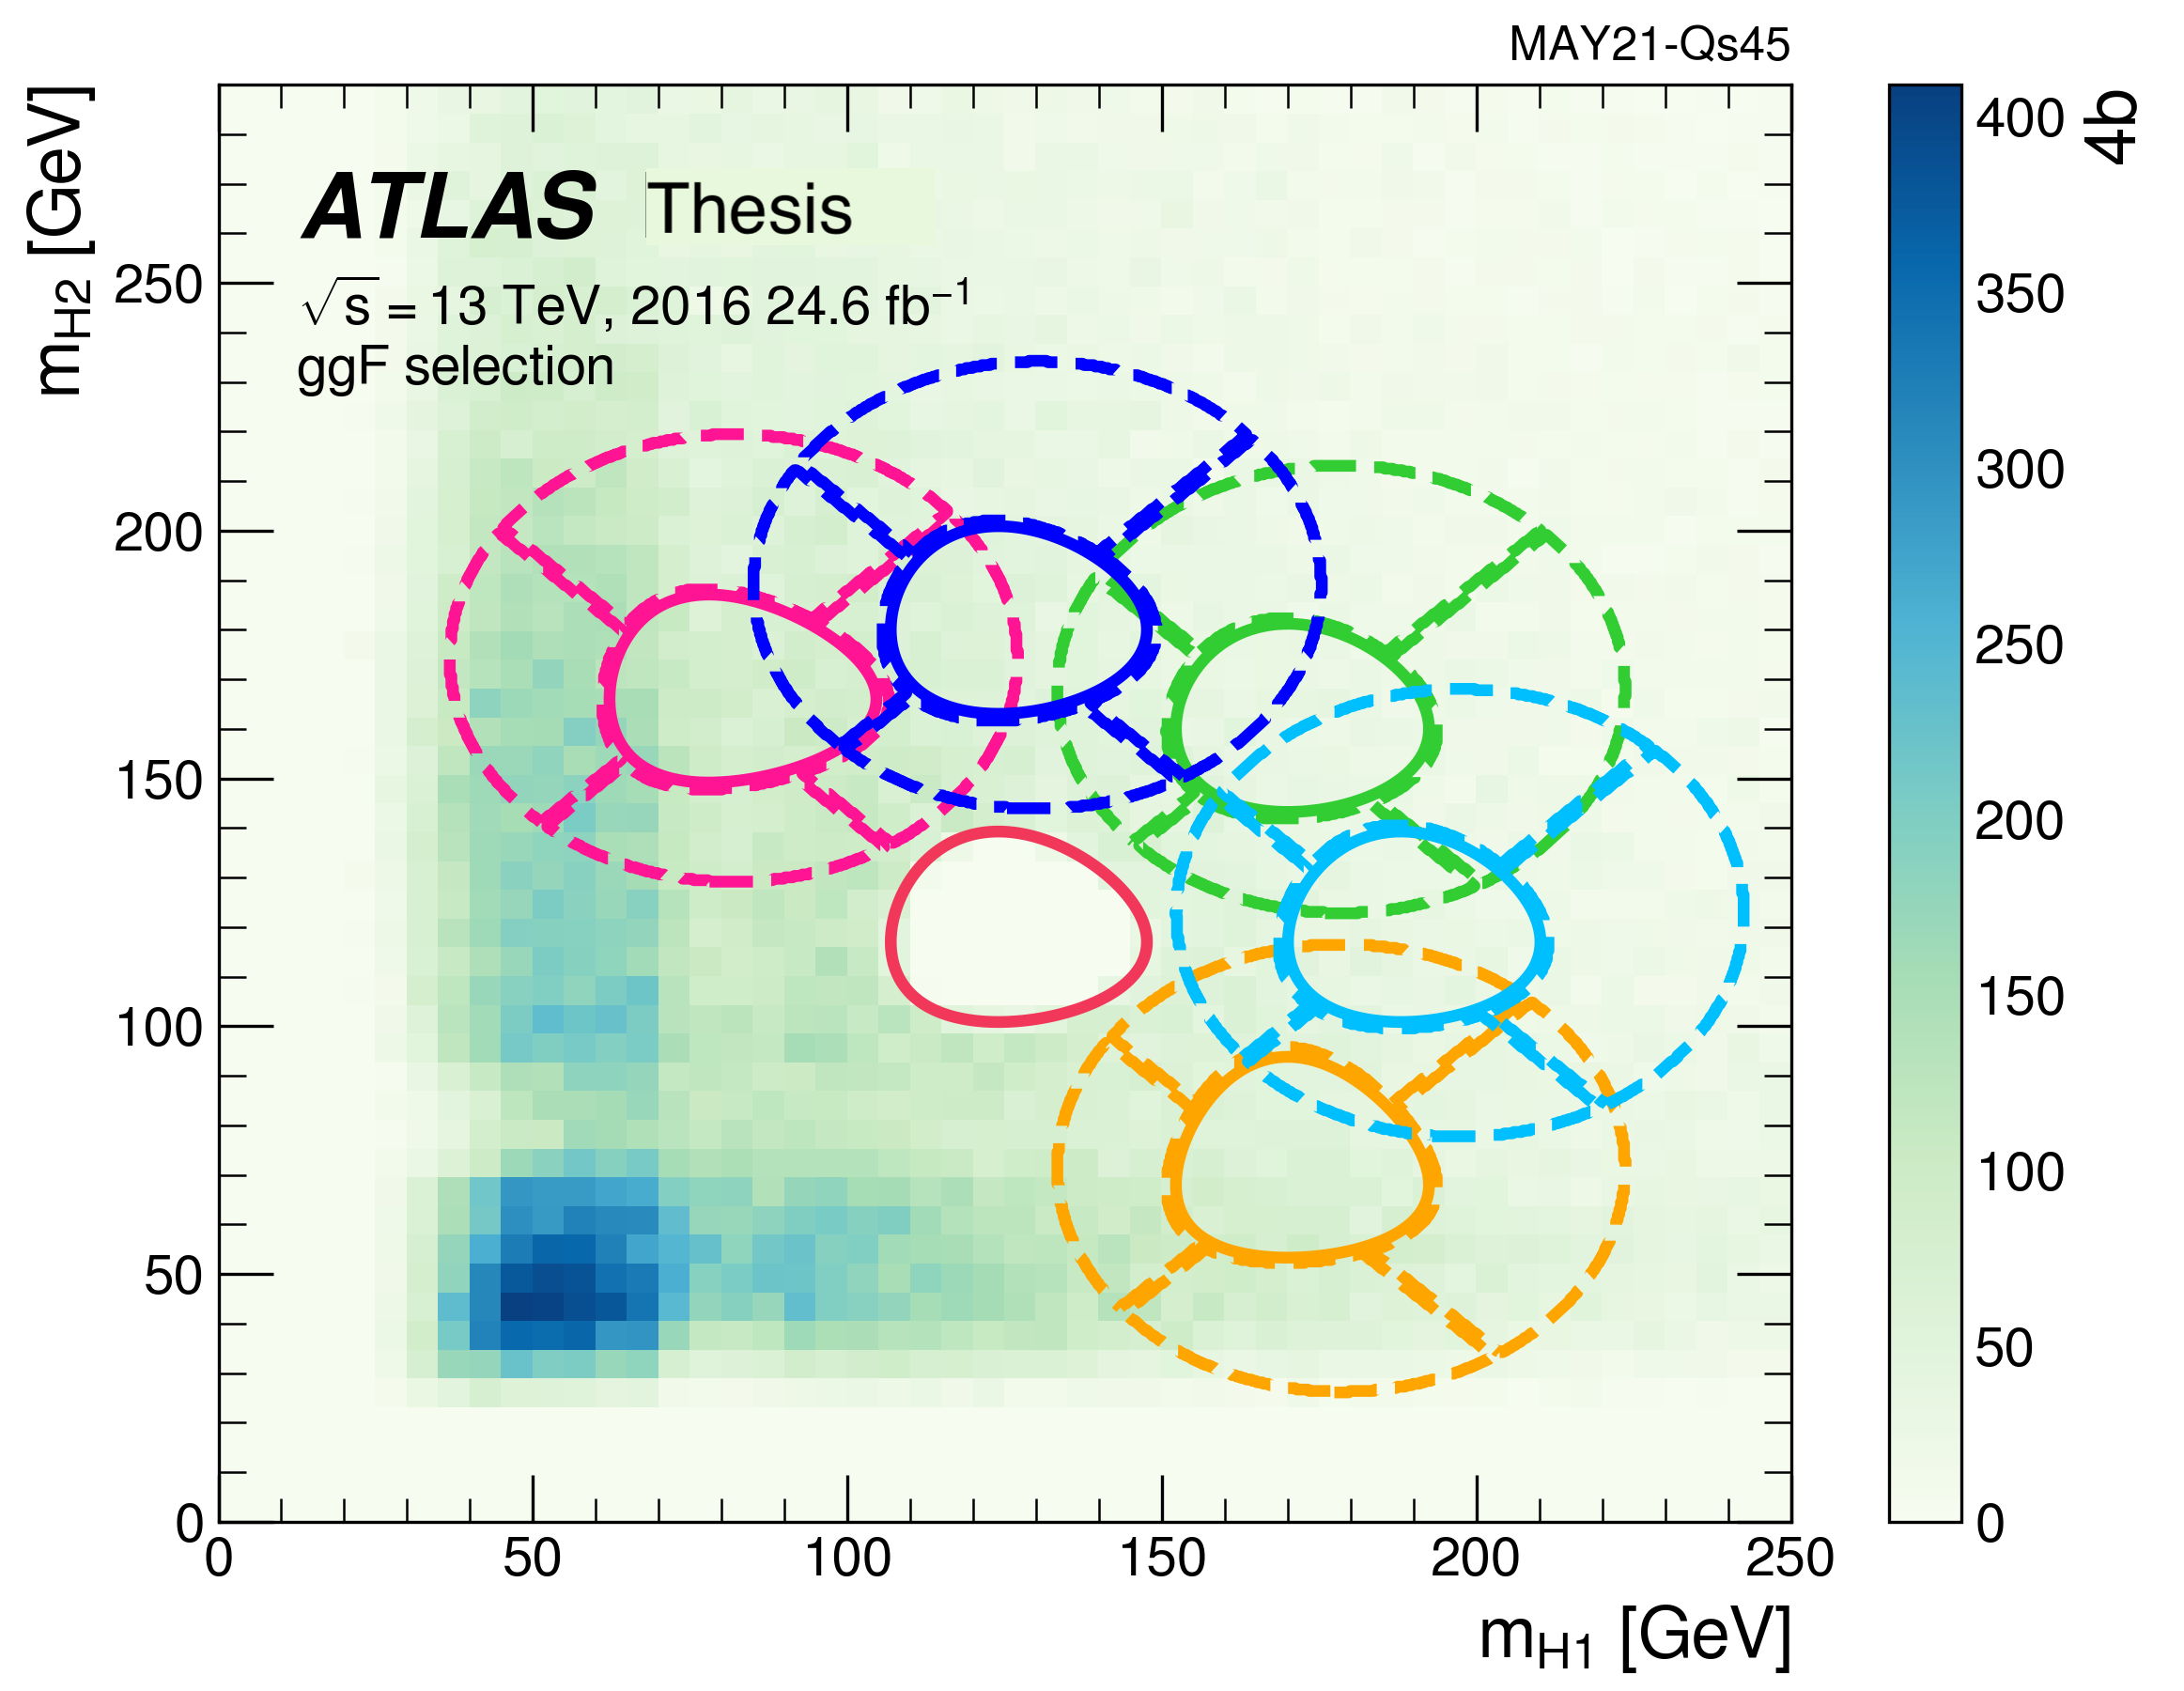
\includegraphics[width=0.65\textwidth]{\figpath/shifted-region/massplane/shifted-regions.png}%
  \caption{The shifted regions for the background validation, with the pink solid curve in the center showing the nominal SR. }
           \label{fig:shifted-regions}
\end{figure}

\begin{table}[htbp]
\centering
\begin{tabular}{ c | c | c | c}
\textbf{(Shifted) Signal Region} & $m_{\PH1}$ center [GeV] &  $m_{\PH2} $ center [GeV] & nominal rw set \\
\hline
\textcolor{deeppink}{upper left} & 78 & 166 & CR1 \\
\textcolor{blue}{upper center} & 124 & 180 & CR1 \\
\textcolor{green}{upper right} & 170 & 166 & CR1 \\
\textcolor{cyan}{center right} & 188 & 117 & CR1 \\
\textcolor{orange}{lower right} & 170 & 68 & CR2 \\
\hline
\textcolor{hh:darkpink}{nominal} & 124 & 117 & CR1 \\
\end{tabular}
\caption{Center locations for the shifted SRs validation study. Also included is which quadrants are considered the ``nominal''  for the background estimate.}
\label{tab:shift-sr-centers}
\end{table}

\def\yr{18}
The reweighting functions were derived for each of these regions and for all of the year dataset, but to exemplify the agreement we were seeing, in \Fig{\ref{fig:bkgd4b-20\yr-shifted-region}} we show the \mhh predictions compared to the observed 4b data. 
In the ratio panels, you can see that there is good agreement already with the given error bars, and gave us confidence in the background estimation procedure that we had set up.

\begin{figure}[ht]
    \centering
    \subfloat[\textcolor{deeppink}{Upper left}]{
    	   \label{fig:mhh-UL-4bSR-20\yr}%
            \includegraphics[width=0.33\textwidth]{\figpath/shifted-region/bkgd-4b-nocat/MAY21-Qs45-MeanWeight-UL-m-hh-Signal-Region-NN-\yr-4binclusive.png}
    }   
    \subfloat[\textcolor{blue}{Upper center}]{
    	\label{fig:mhh-UC-4bSR-20\yr}%
        \includegraphics[width=0.33\textwidth]{\figpath/shifted-region/bkgd-4b-nocat/MAY21-Qs45-MeanWeight-UC-m-hh-Signal-Region-NN-\yr-4binclusive.png}
    }   
    \subfloat[\textcolor{green}{Upper right}]{
    	\label{fig:mhh-UR-4bSR-20\yr}%
        \includegraphics[width=0.33\textwidth]{\figpath/shifted-region/bkgd-4b-nocat/MAY21-Qs45-MeanWeight-UR-m-hh-Signal-Region-NN-\yr-4binclusive.png}
    }   
 
    \subfloat[\textcolor{cyan}{Center right}]{
    	\label{fig:mhh-CR-4bSR-20\yr}%
        \includegraphics[width=0.33\textwidth]{\figpath/shifted-region/bkgd-4b-nocat/MAY21-Qs45-MeanWeight-CR-m-hh-Signal-Region-NN-\yr-4binclusive.png}
    }   
    \subfloat[\textcolor{orange}{Lower right}]{
    	\label{fig:mhh-LR-4bSR-20\yr}
        \includegraphics[width=0.33\textwidth]{\figpath/shifted-region/bkgd-4b-nocat/MAY21-Qs45-MeanWeight-LR-m-hh-Signal-Region-NN-\yr-4binclusive-VRw.png}
    }   
    \caption{$m_{\higgs\higgs}$ distributions of reweighted 2b data and 4b data in the shifted SRs for the 20\yr \ background estimates. 
             The background error bar includes the 2b Poisson, deep ensembles, and the CR1 / CR2 shape difference.}
    \label{fig:bkgd4b-20\yr-shifted-region}
\end{figure}

To further estimate this, a comparison of the predicted and observed yields was made and showed in \Tab{\ref{tab:shifted-4b-yields}}. To quantify the level of agreement between the observation and the predcition, 

\begin{equation}
    \mu_{\mathrm{norm}} = \frac{(N_{\mathrm{bkgd}}-N_{\mathrm{target}})}{\sigma_{\mathrm{stat}}}
    \label{eq:shifted-norm}
\end{equation}

where $\sigma_{stat}$ includes the statistical errors from: the 4b Poisson error (on the obs) the 2b Poisson error (on the background template) and the deep ensembles error (on the background template from retraining 100x)  -- all summed in quadrature. To quantify the difference across the years and regions, \Fig{\ref{shift-norms}} shows a histogram of the deviation $\mu_\mathrm{norm}$, and the Gaussian fit to the $\mu_{norms}$ has a mean of -0.08 and a standard deviation of 1.19, which is close to the mean 0 and standard deviation of 1 corresponding to good modeling.
 
%%%%%%%%%%%%%%%%%%%%
% Include table of norms
%%%%%%%%%%%%%%%%%%%%
\begin{table}[ht]
    \centering
    %\setlength\extrarowheight{5pt}
    \begin{tabular}{ccccc}
        \toprule
            Shifted Region & Year & 4b Yield & Background Prediction & Deviation ($\mu_\mathrm{norm}$)\\
        \midrule
            {}                                       & 2016 & 4068 $\pm$ 64 & 4101.6 $\pm$ 474.4 &  0.07 \\
\textcolor{deeppink}{upper left}    & 2017 & 5586 $\pm$ 75 & 5843.4 $\pm$ 514.3 &  0.50 \\
	    {}                                       & 2018 & 9421 $\pm$ 97 & 9559.7 $\pm$ 1051.2 &  0.13 \\
            \hline
            {}                                         & 2016 & 2197 $\pm$ 47 & 2086.3 $\pm$  52.4 & -1.57 \\
\textcolor{blue}{upper center}  & 2017 & 3017 $\pm$ 55 & 2987.9 $\pm$  72.8 & -0.32 \\
            {}                                         & 2018 & 5161 $\pm$ 72 & 5058.6 $\pm$  141.6 & -0.65 \\
	    \hline
            {}                                        & 2016 & 1182 $\pm$ 34 & 1125.8 $\pm$  38.8 & -1.08 \\
\textcolor{green}{upper right} & 2017 & 1738 $\pm$ 42 & 1684.4 $\pm$  40.2 & -0.93 \\
            {}                                        & 2018 & 2831 $\pm$ 53 & 2732.7 $\pm$   48.4 & -1.37 \\
	    \hline
	    {}                               & 2016 & 1305 $\pm$ 36 & 1310.2 $\pm$  43.6 &  0.09 \\
\textcolor{cyan}{center right} & 2017 & 1922 $\pm$ 44 & 1951.2 $\pm$  73.7 &  0.34 \\
            {}                                & 2018 & 3098 $\pm$ 56 & 3108.0 $\pm$   98.6 &  0.09 \\
	    \hline
            {}                                  & 2016 & 2658 $\pm$ 52 & 2664.2 $\pm$ 300.0 &  0.02 \\
\textcolor{orange}{lower right} & 2017 & 3635 $\pm$ 60 & 3814.4 $\pm$ 326.7 &  0.54 \\
 	    {}                                  & 2018 & 6084 $\pm$ 78 & 6241.1 $\pm$  491.1 &  0.32 \\
        \bottomrule
    \end{tabular}
    \caption{4b and background prediction in the signal region in the shifted regions in 2016. The error of background prediction includes the 2b poisson statistic error, the bootstrap error and the shape systematic error.}
    \label{tab:shifted-4b-yields}
\end{table}

\begin{figure}[ht]
  \centering
  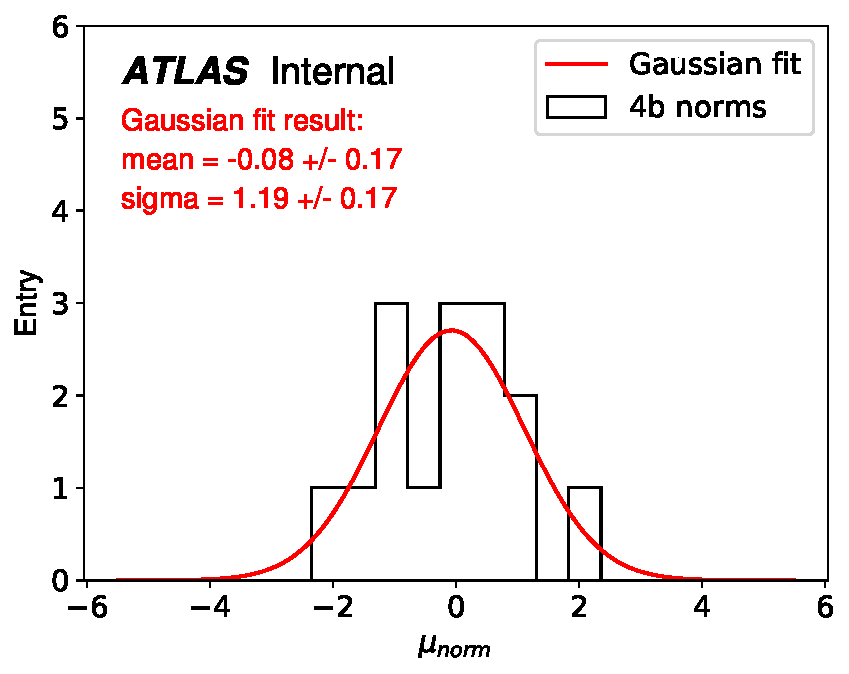
\includegraphics[width=0.60\textwidth]{\figpath/shifted-region/norms/pubnorm.pdf}%
  \caption{$\mu_{\mathrm{norm}}$ distribution in the shifted regions. 
           4b normalizations (black) and the gaussian fit (red) are shown.
           }
  \label{fig:shift-norms} 
\end{figure}

Finally, in \Fig{\ref{fig:shifted-region-pull-plots}} shows the pull plots for the fit with the background nuisance parameters % except the 3b1f syst
to the observed data.
Since the best fit values are within the $1\sigma$ error bands of the inputted templates, this gave us confidence moving forward that our background model well described the shifted SR data, giving us confidence moving forward with unblinding.

\begin{figure}[ht]
    \centering
    \subfloat[\textcolor{deeppink}{upper left}]{%
            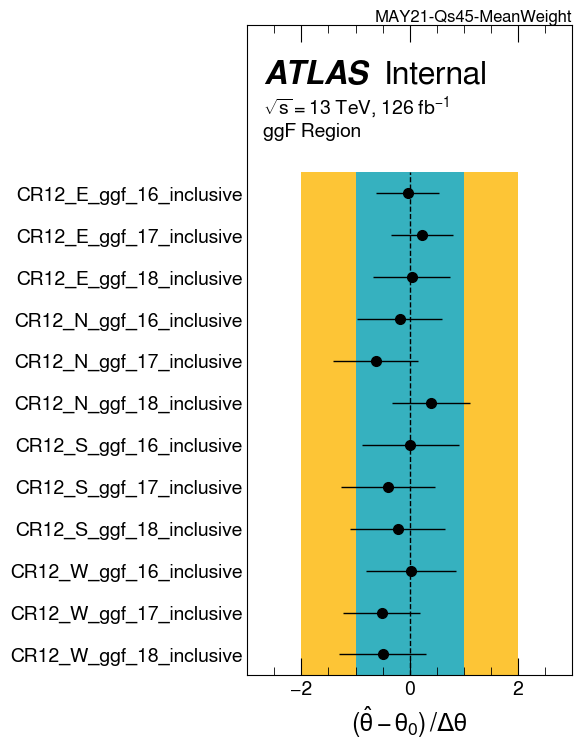
\includegraphics[width=0.25\textwidth]{{\figpath/shifted-region/bonly-pull/shifted_UL_bkg_only_fit_nocat_res_p09_samps_ggf_pd_ggf_161718_mod_kl_1.00_k2v_1.00_k1v_1.00_b_only_Pulls.png}}
    }
    \subfloat[\textcolor{blue}{upper center} ]{%
            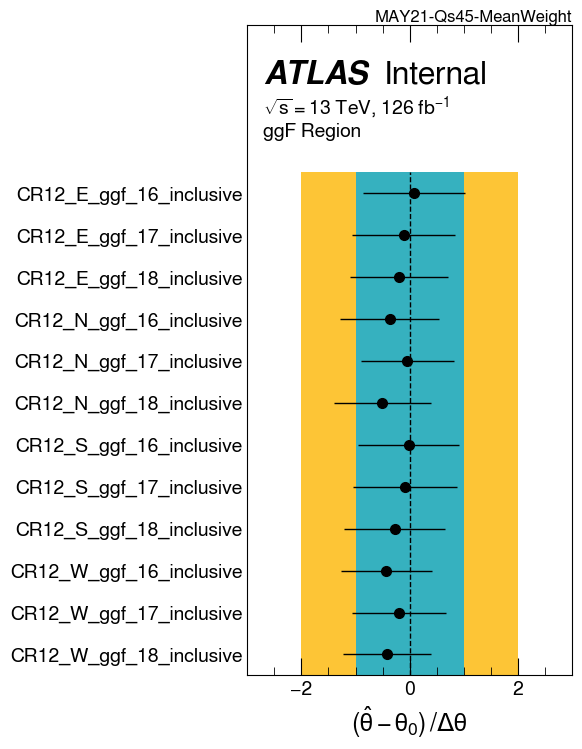
\includegraphics[width=0.25\textwidth]{{\figpath/shifted-region/bonly-pull/shifted_UC_bkg_only_fit_nocat_res_p09_samps_ggf_pd_ggf_161718_mod_kl_1.00_k2v_1.00_k1v_1.00_b_only_Pulls.png}}
    }
    \subfloat[\textcolor{green}{upper right} ]{%
            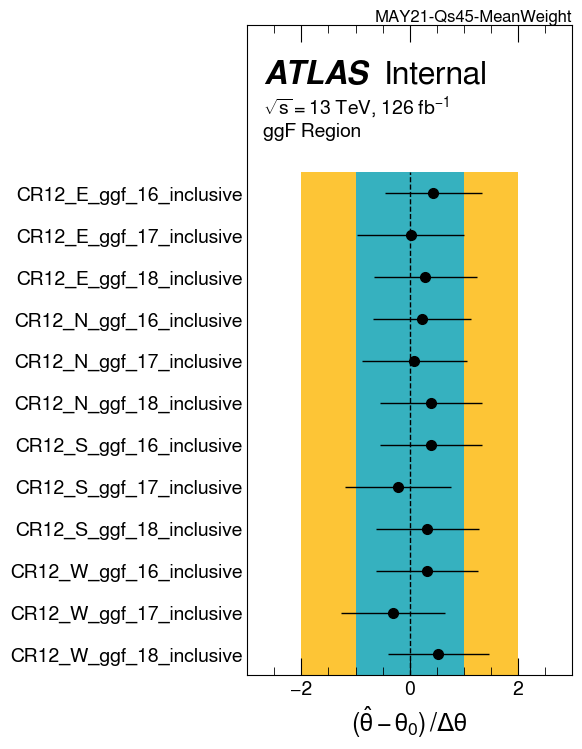
\includegraphics[width=0.25\textwidth]{{\figpath/shifted-region/bonly-pull/shifted_UR_bkg_only_fit_nocat_res_p09_samps_ggf_pd_ggf_161718_mod_kl_1.00_k2v_1.00_k1v_1.00_b_only_Pulls.png}}
    }

    \subfloat[\textcolor{cyan}{center right}]{%
            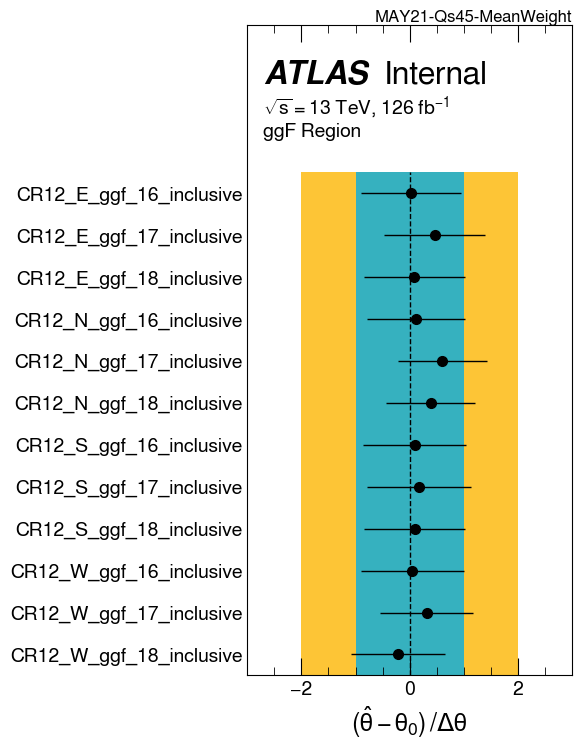
\includegraphics[width=0.25\textwidth]{{\figpath/shifted-region/bonly-pull/shifted_CR_bkg_only_fit_nocat_res_p09_samps_ggf_pd_ggf_161718_mod_kl_1.00_k2v_1.00_k1v_1.00_b_only_Pulls.png}}
    }
    \subfloat[\textcolor{orange}{lower right}]{%
            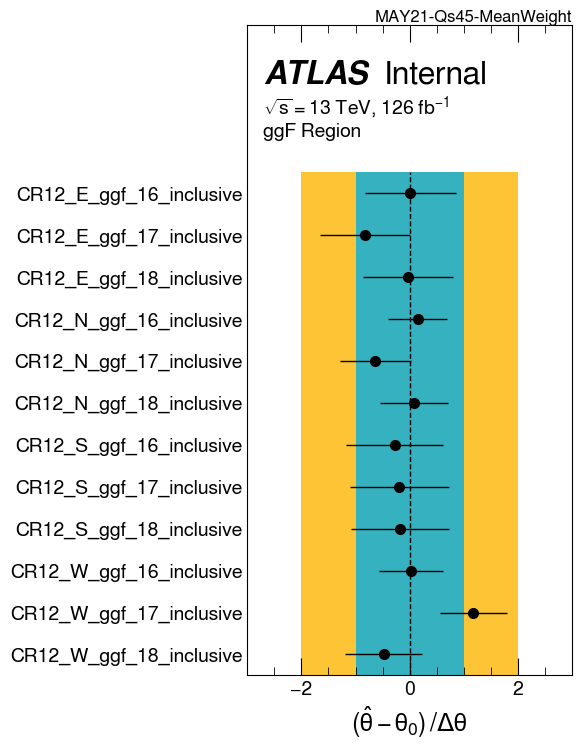
\includegraphics[width=0.25\textwidth]{{\figpath/shifted-region/bonly-pull/shifted_LR_bkg_only_fit_nocat_res_p09_samps_ggf_pd_ggf_161718_mod_kl_1.00_k2v_1.00_k1v_1.00_b_only_Pulls.png}}
    }

    \caption{Background only pull plots in the shifted regions}
    \label{fig:shifted-region-pull-plots}
\end{figure}



\FloatBarrier
\subsection{MC validation}

\begin{itemize}
	\item A monte carlo sample of QCD (with pythia) and \ttbar were also used to test the 4b SR before unblinding. 
\end{itemize}

\textbf{Validate with data trained networks}

%\begin{table}[ht]
%    \centering
%    \caption{The 4b and reweighted 2b yields in QCD and \ttbar MC simulation in SR. The errors on the background prediction include the 2b Poisson statistic error, bootstrap error and shape systematic error.}
%    \setlength\extrarowheight{5pt}
%    \begin{tabular}{cccc}
%        \toprule
%            Year & 4b Yield & Background Prediction & Deviation ($\sigma$) \\
%        \midrule
%            2016 & 3312.6 $\pm$ 227.3 & 2997.2 $\pm$ 208.8 & 1.02 \\
%            2017 & 4835.1 $\pm$ 270.5 & 4551.7 $\pm$ 295.8 & 0.71 \\
%            2018 & 8018.3 $\pm$ 435.3 & 7321.2 $\pm$ 473.5 & 1.08 \\
%        \bottomrule
%    \end{tabular}
%    \label{tbl:mc-4b-yields}
%\end{table}

\begin{figure}[ht]
    \centering
    \subfloat[$m_{\higgs\higgs}$ in 2016]{
    	\label{fig:mhh-4b-2016-mc-bkg}%
        \includegraphics[width=0.33\textwidth]{\figpath/mc-validation/bkgd-4b-nocat/MAY21-Qs45-MeanWeight-MC-m-hh-Signal-Region-NN-16-4binclusive.png}
    }
    \subfloat[$m_{\higgs\higgs}$ in 2017]{
    	\label{fig:mhh-4b-2017-mc-bkg}%
        \includegraphics[width=0.33\textwidth]{\figpath/mc-validation/bkgd-4b-nocat/MAY21-Qs45-MeanWeight-MC-m-hh-Signal-Region-NN-17-4binclusive.png}
    }
    \subfloat[$m_{\higgs\higgs}$ in 2018]{\label{fig:mhh-4b-2018-mc-bkg}%
            \includegraphics[width=0.33\textwidth]{\figpath/mc-validation/bkgd-4b-nocat/MAY21-Qs45-MeanWeight-MC-m-hh-Signal-Region-NN-18-4binclusive.png}
    }
    \caption{$m_{\higgs\higgs}$ \textbf{data reweighted} 2b events and 4b events \textbf{evaluated on the QCD and \ttbar \ MC} samples. 
             The background estimate error includes the 2b poisson, deep ensembles, and CR1/CR2 shape systematic errors.}
    \label{fig:bkgd4b-mc-bkg}
\end{figure}



\textbf{Validate with MC (re)trained networks}

\def\figpath{figures/nr-int-note/appendices/bkgd-mc-validation/V2}

\begin{figure}[ht]
    \centering
    \subfloat[$m_{\higgs\higgs}$ in 2016]{\label{fig:mhh-4b-2016-mcweight-bkg}%
            \includegraphics[width=0.33\textwidth]{\figpath/mc-weights/bkgd-4b-nocat/sig/2016/MAY21-Qs45-MeanWeight-MC-m-hh-Signal-Region-NN-16-4binclusive.png}
    }
    \subfloat[$m_{\higgs\higgs}$ in 2017]{\label{fig:mhh-4b-2017-mcweight-bkg}%
            \includegraphics[width=0.33\textwidth]{\figpath/mc-weights/bkgd-4b-nocat/sig/2017/MAY21-Qs45-MeanWeight-MC-m-hh-Signal-Region-NN-17-4binclusive.png}
    }
    \subfloat[$m_{\higgs\higgs}$ in 2018]{
    	\label{fig:mhh-4b-2018-mcweight-bkg}%
         \includegraphics[width=0.33\textwidth]{\figpath/mc-weights/bkgd-4b-nocat/sig/2018/MAY21-Qs45-MeanWeight-MC-m-hh-Signal-Region-NN-18-4binclusive.png}
    }
    \caption{$m_{\higgs\higgs}$ \textbf{MC reweighted} 2b events and 4b events evaluated on the QCD and \ttbar \ MC samples. 
             The background estimate error includes the 2b poisson, deep ensembles, and CR1/CR2 shape systematic errors.}
    \label{fig:bkgd4b-mcweight-bkg}
\end{figure}

%\begin{table}[ht]
%    \centering
%    \caption{\label{tbl:mcweight-4b-yields} 4b yield and reweighted 2b yield of 
%             QCD and \ttbar MC samples in SR. MC derived weights are used. 
%             The error of background prediction includes 2b poisson statistic 
%             error, bootstrap error and shape systematic error.}
%    \setlength\extrarowheight{5pt}
%    \begin{tabular}{cccc}
%        \toprule
%            year & 4b yield & background prediction & deviation \\
%        \midrule
%            2016 & 3312.6 $\pm$ 227.3 & 2949.4 $\pm$ 233.0 & 1.12 \\
%            2017 & 4835.1 $\pm$ 270.5 & 4746.5 $\pm$ 301.2 & 0.22 \\
%            2018 & 8018.3 $\pm$ 435.3 & 7628.3 $\pm$ 518.9 & 0.58 \\
%        \bottomrule
%    \end{tabular}
%\end{table}




